\chapter{Experiment and Result}
brief of experiment and result.
\section{Experiment}
Please tell how the experiment conducted from method.

\section{Result}
Please provide the result of experiment

\section{Lusia Violita Aprilian/1164080}

\subsection{Teori}
\begin{enumerate}
\item Klasifikasi teks
	\par Klasifikasi Dokumen / Teks adalah salah satu tugas penting dan tipikal dalam supervised machine learning (ML). Menetapkan kategori pada dokumen, yang dapat berupa halaman web, buku perpustakaan, artikel media, galeri, dll. Memiliki banyak aplikasi seperti mis. penyaringan spam, perutean email, analisis sentimen dll. 
	\begin{figure}[ht]
		\centering
		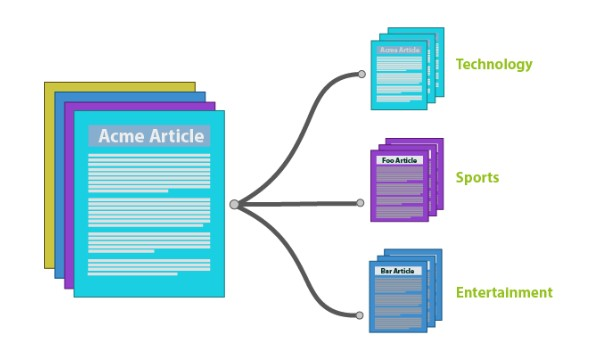
\includegraphics[scale=0.5]{figures/m1.jpg}
		\caption{Lusia-Klasifikasi teks}
		\label{contoh}
	\end{figure}
	
\item Klasifikasi Bunga tidak dapat penggunakan machine learning
	\par Klasifikasi bunga tidak dapat menggunakan machine learning karena memiliki masalah input yang serupa namun output yang berbeda atau 'noise'. Yang dimaksud dengan noise adalah contoh output yang direkam bukan seperti seharusnya. Misalnya saja kita secara implisit berasumsi bahwa contoh bunga kita telah diklasifikasikan dengan benar. Tetapi ini harus dilakukan dengan seseorang yang tepat, seperti seorang ahli botani. Seorang ahli botani ahli harus melihat contoh bunga dan berkata: " ini adalah setosa ... ini adalah virginica ", dan dengan demikian bertindak sebagai "guru" yang memungkinkan mesin untuk belajar. Tetapi bagaimana jika guru itu melakukan kesalahan? Selain itu, selalu ada peluang untuk memperkenalkan kesalahan saat merekam data. Noise juga ditemukan dalam pengukuran, yang selalu sedikit bermasalah karena alat dan sensor kami tidak sempurna dan hanya bekerja pada tingkat presisi tertentu.
	\begin{figure}[ht]
		\centering
		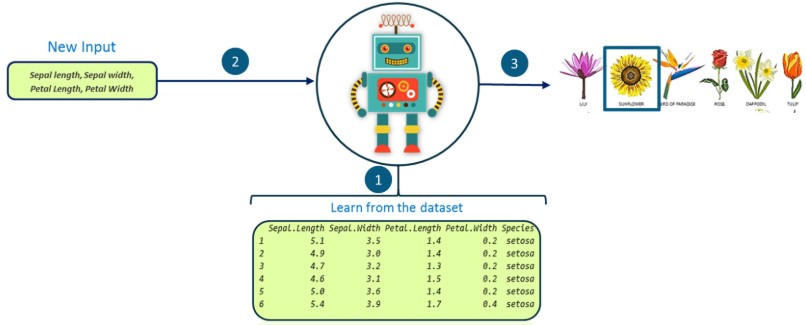
\includegraphics[scale=0.5]{figures/m2.jpg}
		\caption{Lusia-Klasifikasi bunga}
		\label{contoh}
	\end{figure}

\item Teknik pembelajaran mesin pada teks YouTube
	\par Dengan menggunakan kasus seperti rekomendasi video yang terdapat pada fiturnya, Machine Learning pada YouTube memperhatikan apa saja yang menarik perhatian para penggunanya. Ketika kita sedang menonton di YouTube, pada sebelah kanan terdapat 'Up Next' yang menampilkan beberapa video serupa yang sedang ditonton. Dan ketika mengklik salah satu video dari baris tersebut, maka YouTube akan mengingatnya dan menggunakan kata yang tertera sebagai referensi. 
	\begin{figure}[ht]
		\centering
		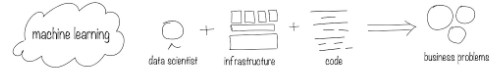
\includegraphics[scale=0.5]{figures/m3.jpg}
		\caption{Lusia-Teknik YouTube}
		\label{contoh}
	\end{figure}

\item Vectorisasi Data
	\begin{itemize}
		\item Maksud dari Vectorisasi Data merupakan Pemecahan dan Pembagian Data.
	\end{itemize}
	
\item Bag of word
	\par Bag-of-words adalah cara untuk merepresentasikan data teks saat memodelkan teks dengan algoritma pembelajaran mesin.
	\begin{figure}[ht]
		\centering
		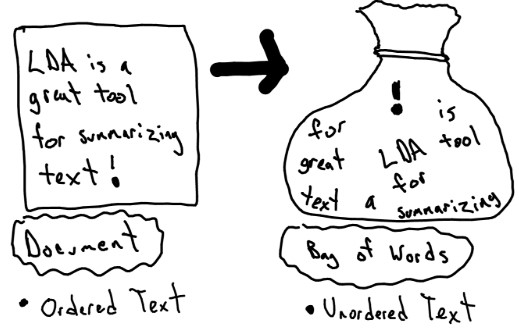
\includegraphics[scale=0.5]{figures/m5.jpg}
		\caption{Lusia-Bag of Word}
		\label{contoh}
	\end{figure}
	
\item TF-IDF
	\par TF-IDF merupakan istilah frekuensi - frekuensi dokumen terbalik, adalah ukuran penilaian yang banyak digunakan dalam pengambilan informasi (IR) atau peringkasan. TF-IDF dimaksudkan untuk mencerminkan seberapa relevan suatu istilah dalam dokumen yang diberikan. Intuisi di baliknya adalah bahwa jika sebuah kata muncul beberapa kali dalam sebuah dokumen, kita harus meningkatkan relevansinya karena itu harus lebih bermakna daripada kata-kata lain yang muncul lebih sedikit kali (TF). Pada saat yang sama, jika sebuah kata muncul berkali-kali dalam suatu dokumen tetapi juga di sepanjang banyak dokumen lain, mungkin itu karena kata ini hanya kata yang sering; bukan karena itu relevan atau bermakna (IDF).
	\begin{figure}[ht]
		\centering
		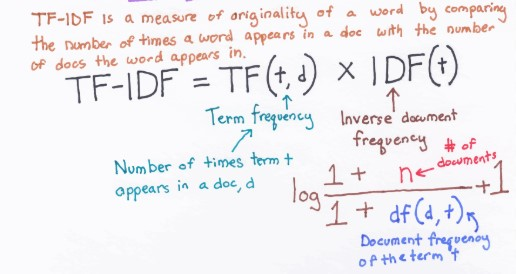
\includegraphics[scale=0.5]{figures/m6.jpg}
		\caption{Lusia-TF IDF}
		\label{contoh}
	\end{figure}
\end{enumerate}

\subsection{Praktek}
\begin{enumerate}
\item Aplikasi menggunakan pandas
	\par Berikut adalah aplikasi yang dibuat menggunakan pandas :
	
		\begin{figure}[ht]
		\centering
		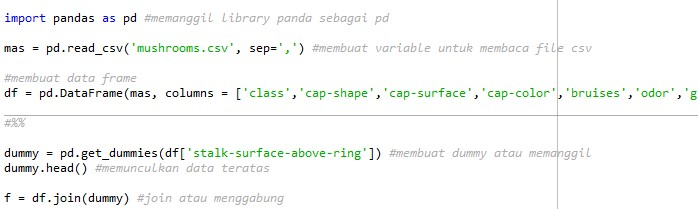
\includegraphics[scale=0.5]{figures/n1a.jpg}
		\caption{Lusia-Pandas}
		\label{contoh}
		\end{figure}
		
	\begin{enumerate}
	\item 1 = memanggil library pandas sebagai pd
	\item 2 = membuat varible mas untuk membaca foile csv
	\item 3 = membuat varible untuk membuat data frame
	\item 4 = membuat variable dummy untuk mengubah kategori menjadi integer
	\item 5 = untuk memunculkan data teratas
	\item 6 = untuk menjoinkan atau menggabungkan data frame dengan dummy
	\end{enumerate}
	
	\par Berikut adalah hasilnya :
	
		\begin{figure}[ht]
		\centering
		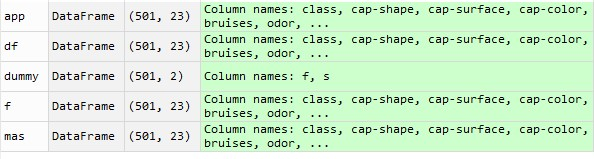
\includegraphics[scale=0.5]{figures/n1b.jpg}
		\caption{Lusia-Hasil Pandas}
		\label{contoh}
		\end{figure}	
	
\item Memecah data frame
	\par Berikut untuk memecah data frame menjadi dua :
	
		\begin{figure}[ht]
		\centering
		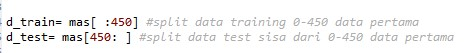
\includegraphics[scale=0.5]{figures/n2a.jpg}
		\caption{Lusia-Pecah data}
		\label{contoh}
		\end{figure}
	
	\begin{enumerate}
	\item 1 = split data training 0-450 data pertama
	\item 2 = split data test sisa dari 0-450 data pertama
	\end{enumerate}
	
	\par Berikut adalah hasilnya :
	
		\begin{figure}[ht]
		\centering
		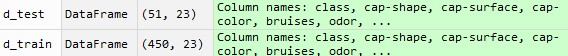
\includegraphics[scale=0.5]{figures/n2b.jpg}
		\caption{Lusia-Hasil Pecah data}
		\label{contoh}
		\end{figure}
		
\item Vektorisasi dan klasifikasi Decission Tree Katty Perry
	\begin{itemize}
	\item Berikut adalah vektorisasi dan klasifikasi Katty Perry
		\begin{figure}[ht]
		\centering
		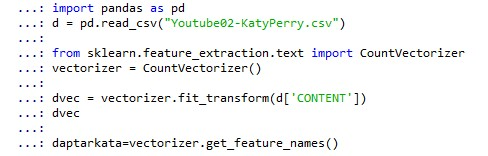
\includegraphics[scale=0.5]{figures/n3a.jpg}
		\caption{Lusia-Vektorisasi dan klasifikasi}
		\label{contoh}
		\end{figure}
	\par Maksud dari gambar vektorisasi dan klasifikasi Katty Perry adalah hasil dari impor dataset, lalu import countvectorizer dari sklearn. Modul sklearn feature extraction digunakan untuk mengekstrak fitur dalam format yang didukung oleh algoritma pembelajaran mesin dari kumpulan data yang terdiri dari format seperti teks dan gambar. Lalu membuat variabel Dan CountVectorizer mengimplementasikan tokenization dan penghitungan kejadian dalam satu kelas. lalu membuat variabel dvec untuk mempelajari dataset. Membuat variabel daptarkata yang berfungsi untuk pemetaan array dari indeks integer fitur ke nama fitur. 
	
	\item Berikut adalah Decission Tree Katty Perry
		\begin{figure}[ht]
		\centering
		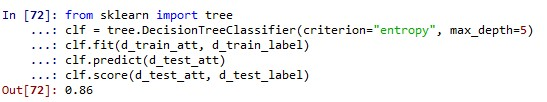
\includegraphics[scale=0.5]{figures/n3b.jpg}
		\caption{Lusia-Decission Tree Katty Perry}
		\label{contoh}
		\end{figure}
	\par Dalam gambar Decission Tree dijelaskan bahwa library tree dari sklearn. Dan mendifinisikan variable untuk memanggil Decission Tree Classifisier yang kemudian dilakukan fit atau pengujian. Lalu menggunakan prediksi dengan fungsi predict untuk memprediksi test. Yang terakhir memunculkan akurasi prediksi yaitu 0,86.
	\end{itemize}

\item Klasifikasikan dari data vektorisasi dengan klasifikasi SVM
	\par Berikut adalah klasifikasikan dari data vektorisasi dengan klasifikasi SVM
		\begin{figure}[ht]
		\centering
		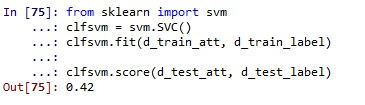
\includegraphics[scale=0.5]{figures/n4.jpg}
		\caption{Lusia-Hasil klasifikasi SVM}
		\label{contoh}
		\end{figure}
	\par Dalam gambar SVM dijelaskan bahwa mula-mula file svm diimpor dari sklearn, lalu melakukan fit dari d train att dan d train label atau disebut dengan pengujian. Selanjutnya variable didifinisikan variable untuk melakukan prediksi dataset dengan SVM. Dan yang terakhir muncul hasilnya yaitu 0,42.
	
\item Klasifikasikan dari data vektorisasi dengan klasifikasi Decission Tree
	\par Maksud dari gambar vektorisasi adalah hasil dari impor dataset
	\par Berikut adalah Decission Tree
		\begin{figure}[ht]
		\centering
		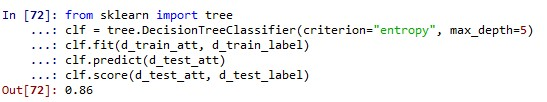
\includegraphics[scale=0.5]{figures/n3b.jpg}
		\caption{Lusia-Decission Tree}
		\label{contoh}
		\end{figure}
	\par Dalam gambar Decission Tree dijelaskan bahwa library tree dari sklearn. Dan mendifinisikan variable untuk memanggil Decission Tree Classifisier yang kemudian dilakukan fit atau pengujian. Lalu menggunakan prediksi dengan fungsi predict untuk memprediksi test. Yang terakhir memunculkan akurasi prediksi yaitu 0,86.

\item Plot confusion matrix
	\par Berikut adalah hasil dari ploting confusion matrix
		\begin{figure}[ht]
		\centering
		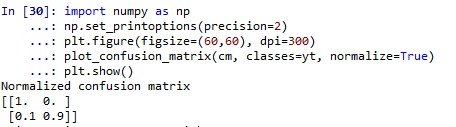
\includegraphics[scale=0.5]{figures/n6.jpg}
		\caption{Lusia-ploting confusion matrix}
		\label{contoh}
		\end{figure}
	\par Dari gambar dijelaskan bahwa library numpy di import sebagai np. Lalu 	Opsi set printoption untuk menentukan cara angka floating point, array dan objek NumPy lainnya ditampilkan. Selanjutnya matplotlib pyplot figure untuk membuat figur atau gambar baru. Selanjutnya confution matrix dinormalisasikan. Dan yang terakhir hasil ditampilkan.

\item Program cross validation
	\par Berikut adalah hasil dari program cross validation
		\begin{figure}[ht]
		\centering
		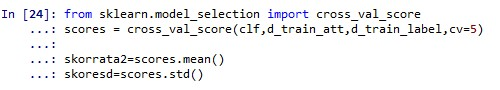
\includegraphics[scale=0.5]{figures/n7.jpg}
		\caption{Lusia-Program cross validation}
		\label{contoh}
		\end{figure}
		
	\par Maksud dari hasil gambar tersebut adalah untuk mendefinisikan dataset untuk 'menguji' model.
	
\item Program pengamatan komponen informasi
	\par Berikut adalah hasil dari program pengamatan komponen informasi
		\begin{figure}[ht]
		\centering
		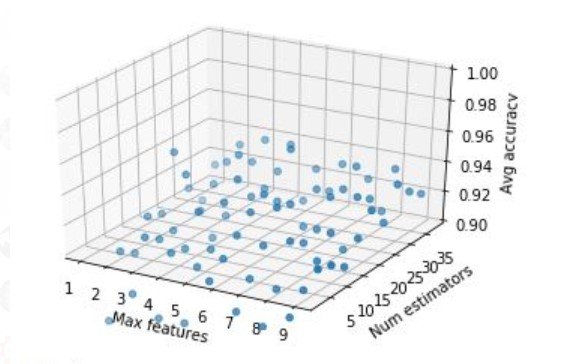
\includegraphics[scale=0.5]{figures/n8.jpg}
		\caption{Lusia-Program pengamatan komponen informasi}
		\label{contoh}
		\end{figure}
		
	\par Maksud dari hasil gambar tersebut adalah diagram informasi dari dataset yang digunakan.

\end{enumerate}

\subsection{Penanganan Error}
\begin{enumerate}
	\item skrinsut error
		\begin{figure}[ht]
		\centering
		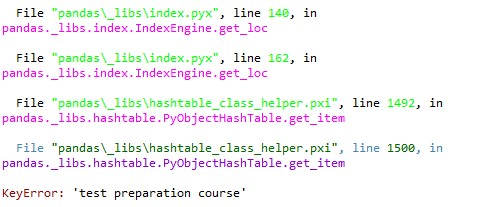
\includegraphics[scale=0.5]{figures/o1.jpg}
		\caption{Lusia-skrinsut error}
		\label{contoh}
		\end{figure}
	\item Tuliskan kode eror dan jenis errornya
		\begin{itemize}
		\item Kode error = KeyError: 'test preparation course'
		\item Jenis error = KeyError
		\end{itemize}
	\item Solusi pemecahan masalah error
		\par Solusinya adalah dengan memasukkan salah satu atribut dari dataset file csv yang digunakan.
\end{enumerate}





\par
\par

\section{Rahmi Roza-1164085}
\subsection{Teori}
Penjelasan Tugas Harian 7 ( No 1-6 )
\begin{enumerate}
\item Pengertian Klasifikasi Teks Dan Ilustrasi Gambar
\begin{itemize}
\item Pengertian Klasifikasi Teks
\par Klasifikasi teks adalah proses proses pengelompokkan bendaberdasarkan ciri-ciri persamaan dan perbedan dengan pemberian tag atau kategori ke teks sesuai dengan isinya. 
\par
\item Ilustrasi Gambar
\par Penjelasan : Berdasarkan pengertian diatas, ada beberapa contoh yang bisa diterapkan. Untuk salah satu contoh dari klasifikasi data sendiri dapat diliat pada gambar berikut \ref{ktRoza}.
\begin{figure}[!hbtp]
\centering
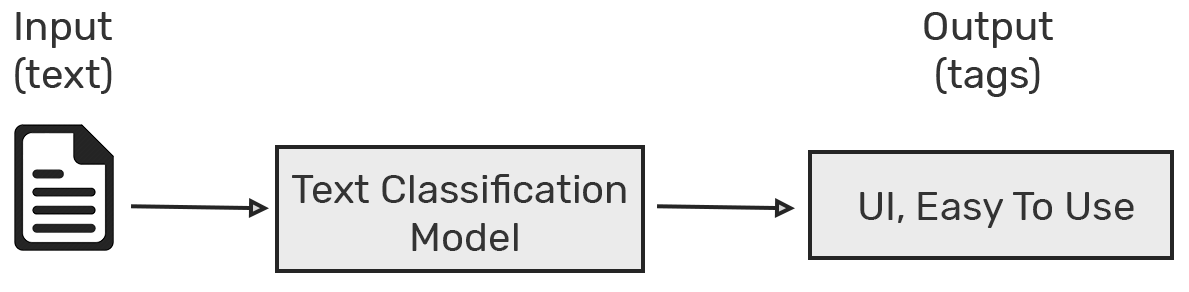
\includegraphics[scale=0.3]{figures/ktRoza.png}
\caption{Klasifikasi Teks Roza}
\label{text-fadila}
\end{figure}
\par
\end{itemize}
\par
\par
\item Mengapa Klasifikasi Bunga Tidak Bisa Menggunakan Machine Learning Dan Ilustrasi Gambar
\begin{itemize}
\item  Mengapa Klasifikasi Bunga Tidak Bisa Menggunakan Machine Learning
\par Penjelasan : Klasifikasi bunga tidak bisa digunakan pada machine learning karena terdapat masalah input yang sama dan output yang berbeda. Output atau error disebut noise.
\par
\item Ilustrasi Gambar
\par Penjelasan : Berdasarkan pengertian diatas, ada beberapa contoh yang bisa diterapkan. Untuk salah satu contoh dari klasifikasi bunga sendiri dapat diliat pada gambar berikut \ref{flowerRoza}.
\begin{figure}[!hbtp]
\centering
\includegraphics[scale=0.3]{figures/flowerRoza.jpg}
\caption{Klasifikasi Bunga Roza}
\label{text-fadila}
\end{figure}
\par
\end{itemize}
\par
\par
\item Teknik Pembelajaran Mesin Pada Teks Pada Kata-Kata Yang Digunakan Di Youtube Dan Ilustrasi Gambar
\begin{itemize}
\item  Teknik Pembelajaran Mesin Pada Teks Pada Kata-Kata Yang Digunakan Youtube
\par Penjelasan : Penggunaan Machine Learning pada Youtube yaitu contohnya pada saat kita melakukan searching vidio atau pun bahan lainnya di youtube maka yang akan ditampilkan adalah vidio dari keyword yang kita ketikkan di kotak pencarian. Dengan kata lain Youtube akan mempfilter vidio dengan keywoard yang telah digunakan. Dan pada saat kita menonton Youtube pada bagian sebelah kanan tampilan youtubr terdapat vidio yang berkaitan dengan keyworad yang kita cari tadi. Dimana disitulah Machine Learning pada Youtube menyimpan data.
\par
\item Ilustrasi Gambar
\par Penjelasan : Berdasarkan pengertian diatas, ada beberapa contoh yang bisa diterapkan. Untuk salah satu contoh dari Mesin Teks Youtube sendiri dapat diliat pada gambar berikut \ref{YoutubeRoza}.
\begin{figure}[!hbtp]
\centering
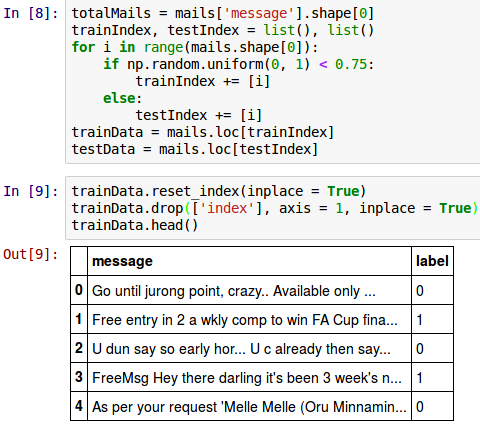
\includegraphics[scale=0.4]{figures/YoutubeRoza.png}
\caption{Youtube Roza}
\label{text-fadila}
\end{figure}
\par
\end{itemize}
\par
\par
\item Vektorisasi Data
\begin{itemize}
\item Maksud Dari Vektorisasi Data
\par Penjelasan : Pembagian dan pemecahan data, dan kemudian dilakukan perhitungan datanya. Vektorisasi juga dapat dimaksudkan dengan setiap data yang mungkin dipetakan ke integer tertentu. Yang mana data tersebut dalam bentuk data vektor diperoleh dalam bentuk koordinat titik yang menampilkan, menempatkan dan menyimpan data spasial dengan menggunakan titik, garis atau area (poligon). 
\par
\end{itemize}

\item Pengertian Bag Of Words Dan Ilustrasi Gambar
\begin{itemize}
\item  Pengertian Bag Of Words
\par Bag Of-Words adalah sebuah konsep yang diambil dari analisis teks yaitu mempresentasikan dokumen sebagai sebuah kantung informasi-infromasi penting tanpa mengurutkan setiap katanya.
\par
\item Ilustrasi Gambar
\par Penjelasan : Berdasarkan pengertian diatas, ada beberapa contoh yang bisa diterapkan. Untuk salah satu contoh dari Bag Of Words sendiri dapat diliat pada gambar berikut \ref{BagofwordsRoza.jpg}.
\begin{figure}[!hbtp]
\centering
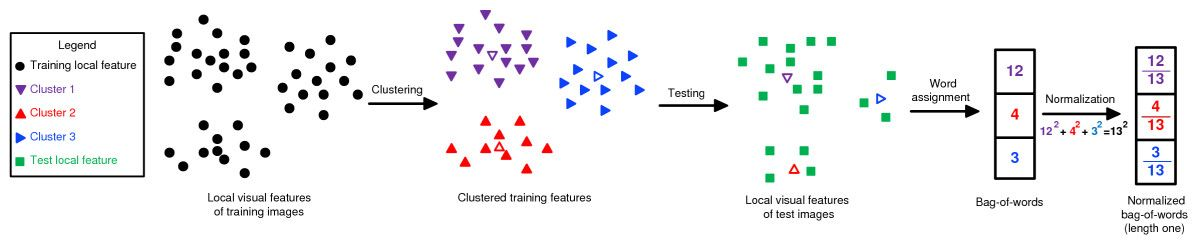
\includegraphics[scale=0.2]{figures/BagofwordsRoza.jpg}
\caption{Bag of Words Roza}
\label{bag-fadila}
\end{figure}
\par
\end{itemize}
\par
\par

\item Pengertian TF-IDF Dan Ilustrasi Gambar
\begin{itemize}
\item  Pengertian TF-IDF
\par TF-IDF  (Term Frequency – Inverse Document Frequency) adalah  sebuah algoritma  adalah salah satu algoritma yang dapat digunakan untuk menganalisa hubungan antara sebuah frase/kalimat dengan sekumpulan dokumen. 
\par Inti utama dari algoritma ini adalah melakukan perhitungan nilai TF dan nilai IDF dari sebuah setiap kata kunci terhadap masing-masing dokumen. Nilai TF dihitung dengan rumus TF = jumlah frekuensi kata terpilih / jumlah kata dan nilai IDF dihitung dengan rumus IDF = log(jumlah dokumen / jumlah frekuensi kata terpilih). Selanjutnya adalah melakukan perkalian antara nilai TF dan IDF untuk mendapatkan jawaban akhir.
\item Ilustrasi Gambar
\par Penjelasan : Berdasarkan pengertian diatas, ada beberapa contoh yang bisa diterapkan. Untuk salah satu contoh dari TF-IDF sendiri dapat diliat pada gambar berikut \ref{TFIDFroza.jpeg}.
\begin{figure}[!hbtp]
\centering
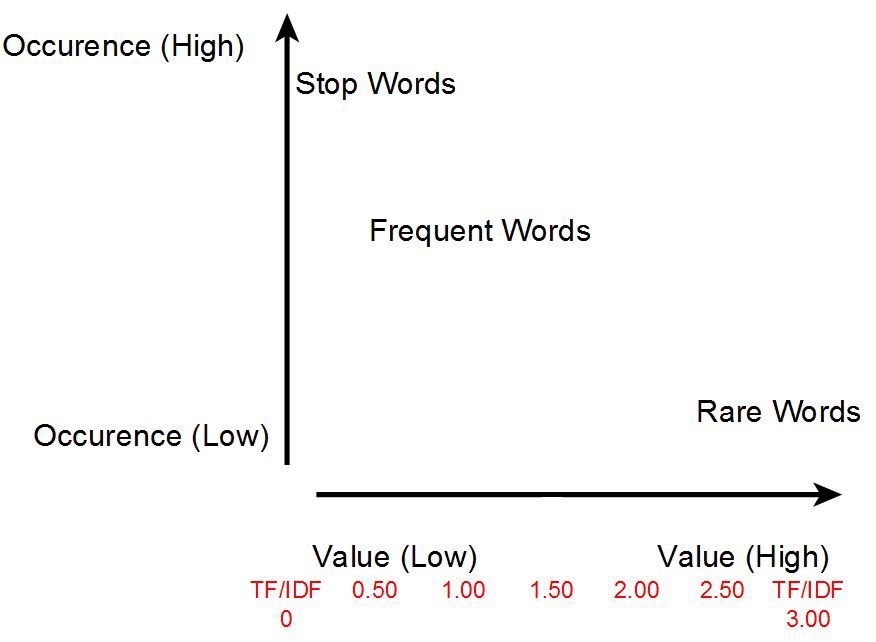
\includegraphics[scale=0.2]{figures/TFIDFroza.jpeg}
\caption{TF-ID Rroza}
\label{tf-fadila}
\end{figure}
\par
\end{itemize}
\par
\par

\subsection{Praktek}
\begin{enumerate}
\item Membuat Aplikasi Sederhana menggunakan pandas, dan membuat data dummy sebnayak 500 baris dan melakukan data load ke data frame panda. Jelaskan arti perbaris!
\begin{figure}[!hbtp]
\centering
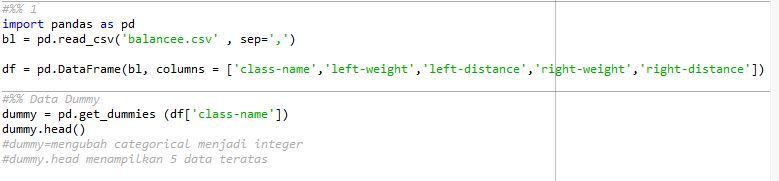
\includegraphics[scale=0.8]{figures/kodinganroza1.jpg}
\caption{Nomor 1 Roza}
\label{text-fadila}
\end{figure}
\begin{itemize}
\item Baris 1: Memanggil library pandas sebagai pd
\item Baris 2: Membaca dataset Balance Scale 
\item Baris 3:Mengambil data frame dari library pandas
\item Baris 4: Data Dummy digunakan untuk mengubah Categorical menjadi Integer
\item Baris 5: Menampilkan 5 data teratas
\par
\end{itemize}
\item GAMBAR HASIL No1:
\begin{figure}[!hbtp]
\centering
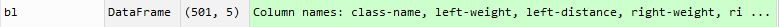
\includegraphics[scale=0.7]{figures/hasil1a.jpg}
\caption{Hasil 1 Roza}
\label{text-fadila}
\end{figure}
\begin{figure}[!hbtp]
\centering
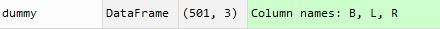
\includegraphics[scale=0.9]{figures/hasil1b.jpg}
\caption{Hasil 1 Roza}
\label{text-fadila}
\end{figure}
\par

\item Membuat Aplikasi Sederhana menggunakan pandas, dan membuat data dummy sebnayak 500 baris dan melakukan data load ke data frame panda. Jelaskan arti perbaris.
\begin{itemize}
\begin{figure}[!hbtp]
\centering
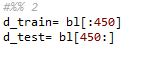
\includegraphics[scale=0.7]{figures/kodinganroza2.jpg}
\caption{Nomor 2 Roza}
\label{text-fadila}
\end{figure}
\item Baris 1: Membagi data set balance scale dari 500 data menjadi data train menjadi 450 data.
\item Baris 2: Membagi data set balance scale dari sisa pembagian data train menjadi data test menjadi 50 data.
\par
\begin{figure}[!hbtp]
\centering
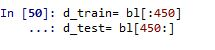
\includegraphics[scale=0.5]{figures/hasil2roza.jpg}
\caption{Hasil 2 Roza}
\label{text-fadila}
\end{figure}
\end{itemize}
\par

\item Vektorisasi dan Klasifikasi Data Dengan Decission Tree
\begin{itemize}
\begin{figure}[!hbtp]
\centering
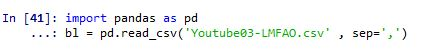
\includegraphics[scale=0.7]{figures/kodinganroza3.jpg}
\caption{Nomor 3 Roza}
\label{text-fadila}
\end{figure}
\begin{figure}[!hbtp]
\centering
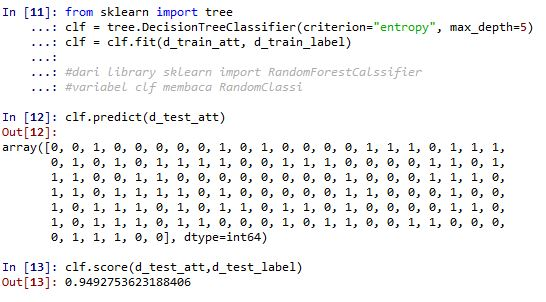
\includegraphics[scale=0.7]{figures/kodinganroza3_.jpg}
\caption{Hasil 3 Roza}
\label{text-fadila}
\end{figure}
\item Penjelasan:
\item Dalam in 11 impor tree dari sklearn. Dan mendefinisikan variabel clf untuk memanggil Decission Tree Classifier dan melakukan fit atau pengujian.
\item Dalam in 12 menggunakan prediksi untk clf dengan function predict untuk memprediksi test. Dan hasilnya muncul dalam bentuk array.
\item clf score memunculkan akurasi prediksi yang dilakukan terhadap clf
\end{itemize}
\par

\item Klasifikasi SVM
\begin{itemize}
\begin{figure}[!hbtp]
\centering
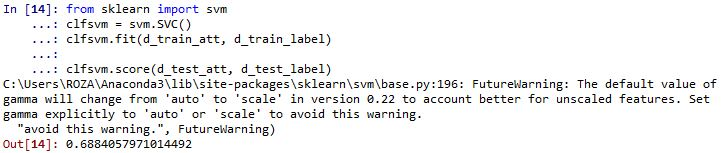
\includegraphics[scale=0.7]{figures/kodinganroza4.jpg}
\caption{Nomor 4 Roza}
\label{text-fadila}
\end{figure}
\item Import SVM dari  sklearn
\item Melakukan fit dari d train att dan d train label atau disebut denga pengujian
\item Mendefinisikan variabel df untuk melakukan prediksi dataset Youtube LMFAO dengan SVM. Dan akan muncul hasil prediksinya 
\end{itemize}
\par

\item Klasifikasi Decision Tree
\begin{itemize}
\begin{figure}[!hbtp]
\centering
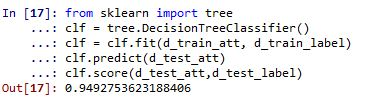
\includegraphics[scale=0.9]{figures/kodinganroza5.jpg}
\caption{Nomor 5 Roza}
\label{text-fadila}
\end{figure}
\item Penjelasan:
\item Dalam in 17 impor tree dari sklearn. Dan mendefinisikan variabel clf untuk memanggil Decission Tree Classifier dan melakukan fit atau pengujian.
\item menggunakan prediksi untk clf dengan function predict untuk memprediksi test. Dan hasilnya muncul dalam bentuk array.
\item clf score memunculkan akurasi prediksi yang dilakukan terhadap clf
\end{itemize}
\par

\item Matplotlib
\begin{itemize}
\begin{figure}[!hbtp]
\centering
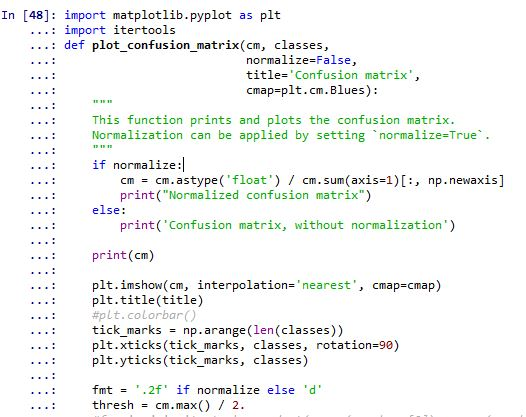
\includegraphics[scale=0.5]{figures/kodinganroza6.jpg}
\caption{Nomor 6 Roza}
\label{text-fadila}
\end{figure}
\item Penjelasan:
\par Fungsi ini mencetak dan memplot Confussion Matrix. Normalisasi dapat diterapkan dengan mengatur `normalize = True`. Ada Confussion Matrik menggunakan normalisasi dan ada confussion matrik tidak menggunakan normalisasi.
\end{itemize}
\par

\item Menjelaskan Program Cross Validation
\begin{itemize}
\begin{figure}[!hbtp]
\centering
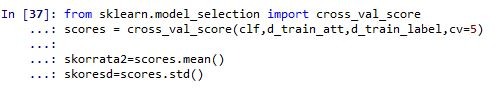
\includegraphics[scale=0.5]{figures/kodinganroza7.jpg}
\caption{Nomor 7 Roza}
\label{text-fadila}
\end{figure}
\item Penjelasan: Variabel score akan melakukan cross validation pada variabel clf, d train att, dan train label. Variabel skorrata2 akan menghitung nilai rata-rata dari  variabel scores tadi menggunakan function mean. Dan scoresd menghitung standar deviasi dari data yang diberikan.
\par
\item GAMBAR HASIL No7:
\begin{figure}[!hbtp]
\centering
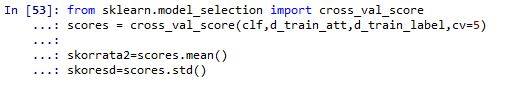
\includegraphics[scale=0.5]{figures/hasilno7.jpg}
\caption{Hasil 7 Roza}
\label{text-fadila}
\end{figure}
\begin{figure}[!hbtp]
\centering
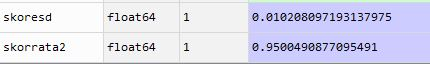
\includegraphics[scale=0.5]{figures/hasilno7b.jpg}
\caption{Hasil 7 Roza}
\label{text-fadila}
\end{figure}
\end{itemize}
\par

\item Program Pengamatan Komponen
\begin{itemize}
\begin{figure}[!hbtp]
\centering
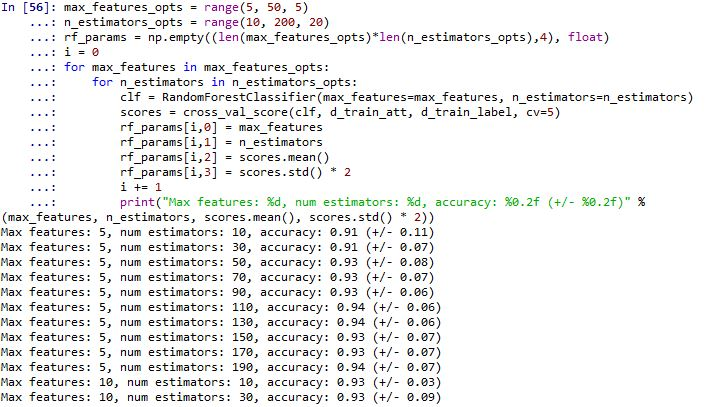
\includegraphics[scale=0.5]{figures/kodingan8.jpg}
\caption{Nomor 8 Roza}
\label{text-fadila}
\end{figure}
\begin{figure}[!hbtp]
\centering
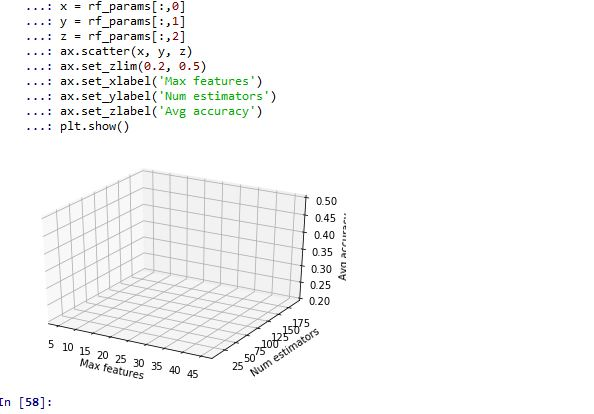
\includegraphics[scale=0.5]{figures/kodinganroza8.jpg}
\caption{Nomor 8 Roza}
\label{text-fadila}
\end{figure}
\item Penjelasan: Pada gambar pertama merupakan kodingan untuk mencetak data dari maxfeatures, num estimators dan accuracy. Sedangkan pada gambar yang kedua itu merupakan gambarnya. Atau hasil gambarnya.
\par 
\end{itemize}
\par

\subsection{Penanganan Error}
\begin{enumerate}
\item Skrinsut Error
\begin{figure}[ht]
\centering
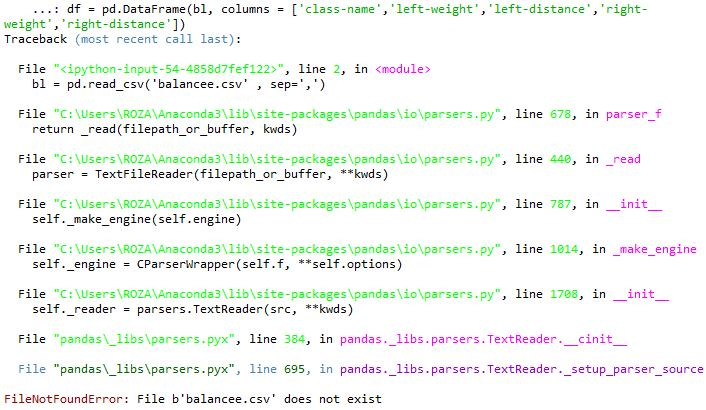
\includegraphics[scale=0.5]{figures/erorque.jpg}
\caption{ Error Roza}
\label{6}
\end{figure}
\item Kode Error dan Jenis Errornya
\par Kode Error: "FileNotFoundError" dan "File b 'balancee.csv' does not exist". 
\par Jenis Error: Import Dataset
\item Penanganan
\par Import ulang dataset dan sesuaikan dengan letak dataset pada file explorer.

\end{enumerate}
\end{enumerate}

\end{enumerate}





\par
\par
\section{Fadila-1164072}
\subsection{Teori}
Penjelasan Tugas Harian 7 ( No 1-6 )
\begin{enumerate}
\item Pengertian Klasifikasi Teks Dan Ilustrasi Gambar
\begin{itemize}
\item Pengertian Klasifikasi Teks
\par Klasifikasi teks adalah proses pemberian tag atau kategori ke teks sesuai dengan isinya. Teks dapat menjadi sumber informasi yang sangat kaya, tetapi mengekstraksi wawasan darinya bisa sulit dan memakan waktu karena sifatnya yang tidak terstruktur.
\par
\item Ilustrasi Gambar
\par Penjelasan : Berdasarkan pengertian diatas, ada beberapa contoh yang bisa diterapkan. Untuk salah satu contoh dari klasifikasi data sendiri dapat diliat pada gambar berikut \ref{text-fadila}.
\begin{figure}[!hbtp]
\centering
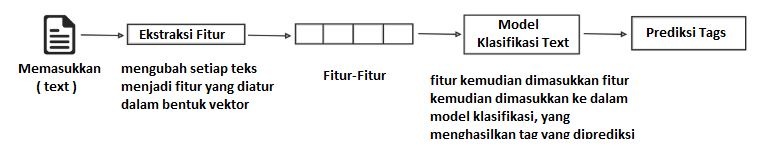
\includegraphics[scale=0.3]{figures/text-fadila.jpg}
\caption{text-fadila}
\label{text-fadila}
\end{figure}
\par
\end{itemize}
\par
\par
\item Mengapa Klasifikasi Bunga Tidak Bisa Menggunakan Machine Learning Dan Ilustrasi Gambar
\begin{itemize}
\item  Mengapa Klasifikasi Bunga Tidak Bisa Menggunakan Machine Learning
\par Penjelasan : Untuk klasifikasi bunga tidak dapat menggunakan machine learning dikarenakan memiliki masalah input yang sama namun keluarannya (output) yang berbeda, biasanya output atau error ini disebut dengan istilah 'noise'. Noise sendiri merupakan output yang disimpan / ditangkap maupun direkam bukan seperti seharusnya ( keluaran yang diiginkan ). 
\par Apabila diberikan contoh, maka contohnya yaitu kita berasumsi secara implisit bahwa klarifikasi bunga yang kita lakukan sudah tepat dan kita melakukannya seperti seorang ahli tanaman. Namun pada hasilnya masih saja terjadi kesalahan. Selain itu, selalu ada peluang untuk memperkenalkan kesalahan saat merekam ataupun menyimpan data, maka harus dilakukan penelitian yang lebih rinci sehingga tidak menimbulkan 'noise' itu sendiri.
\par
\item Ilustrasi Gambar
\par Penjelasan : Berdasarkan pengertian diatas, ada beberapa contoh yang bisa diterapkan. Untuk salah satu contoh dari klasifikasi bunga sendiri dapat diliat pada gambar berikut \ref{bunga-fadila}.
\begin{figure}[!hbtp]
\centering
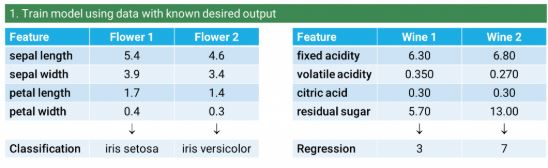
\includegraphics[scale=0.3]{figures/bunga-fadila.jpg}
\caption{bunga-fadila}
\label{bunga-fadila}
\end{figure}
\par
\end{itemize}
\par
\par
\item Teknik Pembelajaran Mesin Pada Teks Pada Kata-Kata Yang Digunakan Di Youtube Dan Ilustrasi Gambar
\begin{itemize}
\item  Teknik Pembelajaran Mesin Pada Teks Pada Kata-Kata Yang Digunakan Youtube
\par Penjelasan : Kita ambil sebuah kasus yang semua orang telah ketahui dan juga pahami. Kasus tersebut yaitu perekomendasian video dari pencarian menggunakan "text / kata" di  Youtube. Pada saat menggunakan Youtube terdapat Machine Learning yang bekerja dan memproses perintah ataupun aktivitas tersebut, dimana akan memfilter secara otomatis video yang disesuaikan dengan "keyword" yang kita masukkan sehingga memberikan keluaran video dengan keyword yang benar. 
\par Adapula fitur yang di dapatkan ketika sedang menonton Youtube. Tampilan sebelah kanan terdapat pilihan 'Next' atapun 'Suggestion' yang menam-pilkan beberapa video serupa sesuai dengan yang dicari atau sedang ditonton. Ketika mengklik salah satu video dari baris tersebut, maka Youtube akan mengingat dan menggunakan kata yang tertera sebagai referensi kembali sehingga akan memberikan kemudahan pada pencarian yang lainnya, Dan disitulah mesin belajar sendiri dan menyimpan data secara berkala sehingga berkembang. 
\par
\item Ilustrasi Gambar
\par Penjelasan : Berdasarkan pengertian diatas, ada beberapa contoh yang bisa diterapkan. Untuk salah satu contoh dari Mesin Teks Youtube sendiri dapat diliat pada gambar berikut \ref{youtube-fadila}.
\begin{figure}[!hbtp]
\centering
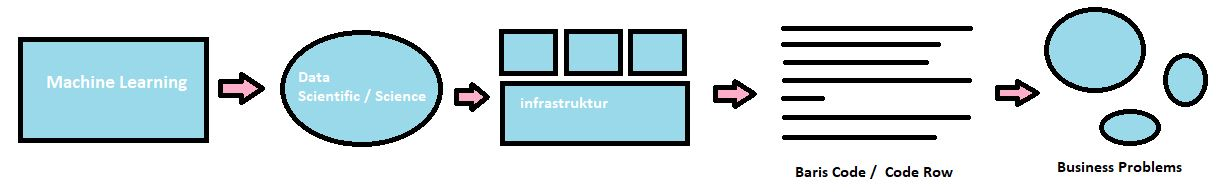
\includegraphics[scale=0.25]{figures/youtube-fadila.jpg}
\caption{youtube-fadila}
\label{youtube-fadila}
\end{figure}
\par
\end{itemize}
\par
\par
\item Vektorisasi Data
\begin{itemize}
\item Maksud Dari Vektorisasi Data
\par Penjelasan : Pembagian dan pemecahan data, kemudian dilakukan perhitungan. Vektorisasi juga dapat dimaksudkan dengan setiap data yang mungkin dipetakan ke integer tertentu. jika kita memiliki array yang cukup besar maka setiap kata / data cocok dengan slot unik dalam array (nilai pada indeks adalah nomor satu kali kata itu muncul).
\par Array angka floating point ( Mewakili data ) :
\begin{itemize}
\item teks
\item audio
\item gambar
\end{itemize}
\par Contoh : -[1.0, 0.0, 1.0, 0.5]
\par
\end{itemize}
\par
\par
\item Pengertian Bag Of Words Dan Ilustrasi Gambar
\begin{itemize}
\item  Pengertian Bag Of Words
\par bag-of-words adalah representasi penyederhanaan yang digunakan dalam pemrosesan bahasa alami dan pengambilan informasi. Model bag-of-words sederhana untuk dipahami dan diterapkan dan telah melihat kesuksesan besar dalam masalah seperti pemodelan bahasa dan klasifikasi dokumen ( penyelesaian dll ).
\par
\par
\item Ilustrasi Gambar
\par Penjelasan : Berdasarkan pengertian diatas, ada beberapa contoh yang bisa diterapkan. Untuk salah satu contoh dari Bag Of Words sendiri dapat diliat pada gambar berikut \ref{bag-fadila}.
\begin{figure}[!hbtp]
\centering
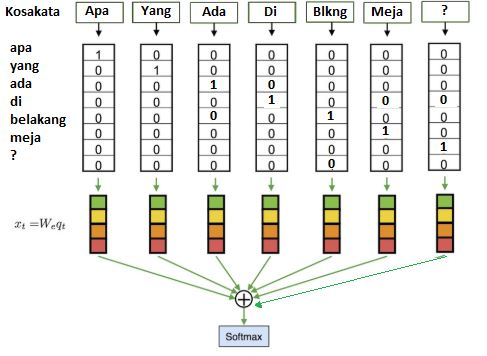
\includegraphics[scale=0.3]{figures/bag-fadila.jpg}
\caption{bag-fadila}
\label{bag-fadila}
\end{figure}
\par
\end{itemize}
\par
\par
\item Pengertian TF-IDF Dan Ilustrasi Gambar
\begin{itemize}
\item  Pengertian TF-IDF
\par TF-IDF atau TFIDF, adalah kependekan dari istilah frekuensi dokumen terbalik, dimana merupakan statistik numerik yang dimaksudkan untuk mencerminkan betapa pentingnya sebuah kata untuk sebuah dokumen dalam kumpulan atau kumpulan.
\par Nilai tf-idf meningkat secara proporsional dengan berapa kali sebuah kata muncul dalam dokumen dan diimbangi dengan jumlah dokumen dalam korpus yang mengandung kata, yang membantu menyesuaikan fakta bahwa beberapa kata muncul lebih sering secara umum
\item Ilustrasi Gambar
\par Penjelasan : Berdasarkan pengertian diatas, ada beberapa contoh yang bisa diterapkan. Untuk salah satu contoh dari TF-IDF sendiri dapat diliat pada gambar-gambar berikut \ref{tf2-fadila}.
\begin{figure}[!hbtp]
\centering
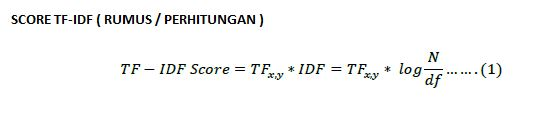
\includegraphics[scale=0.4]{figures/tf2-fadila.jpg}
\caption{tf2-fadila}
\label{tf2-fadila}
\end{figure}
\par
\par
\end{itemize}
\par
\par

\end{enumerate}


\par
\par
\subsection{Praktek Fadila}
Pengerjaanya Tugas Harian 8 ( No 1-8 )
\begin{enumerate}
\item Pembuatan Aplikasi Pandas Sederhana Dengan Menggunakan Dataset berisi 500 baris data.
\begin{itemize}
\item Penjelasan Code Pandas Sederhana
\begin{lstlisting}
import pandas as pd
fadila_car = pd.read_csv('1.csv', sep=';')
len(fadila_car)

fadila = pd.DataFrame(fadila_car, columns = ['buying', 'maint', 'doors', 'persons', 'lug-boot', 'safety', 'class'])

dummy = pd.get_dummies (fadila['class'])
dummy.head()
\end{lstlisting}
\begin{enumerate}
\item Baris 1 : Mengimport Library Pandas sebagai pd
\item Baris 2 : Membuat variabel fadila\_car dimana membaca dataset berupa format csv "1.csv" dengan separator.
\item Baris 3 : Menampilkan hasil dari variabel fadila\_car ( berupa jumlah/angka karena len )
\item Baris 4 : Membuat variabel fadila dimana mengambil/ memanggil DataFrame dari library pd ( pandas ) dengan parameter variabel.
\item Baris 5 : Mendefinisikan variabel dummy dimana memanggil get\_dummies dari pd dengan parameter variabel fadila dan column class
\item Baris 6 : Menampilkan 5 data teratas pada kolom class dari variabel fadila
\end{enumerate}
\item Hasil Dari Aplikasi Sederhana Code Pandas
\par Penjelasan : Hasilnya dapat diliat pada gambar berikut \ref{1-fadila}, \ref{lanjutan1-fadila}, \ref{lanjutan1-1-fadila} dan \ref{lanjutan1-2-fadila}.
\begin{figure}[!hbtp]
\centering
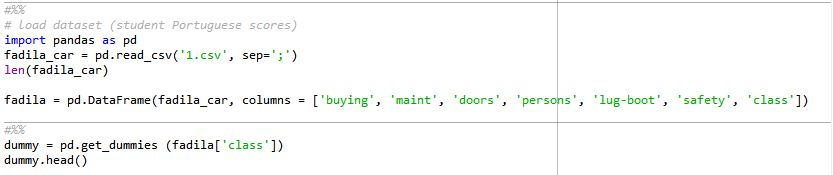
\includegraphics[scale=0.3]{figures/1-fadila.jpg}
\caption{1-fadila}
\label{1-fadila}
\end{figure}
\par
\par
\begin{figure}[!hbtp]
\centering
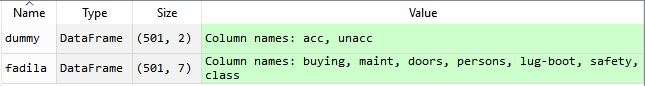
\includegraphics[scale=0.3]{figures/lanjutan1-fadila.jpg}
\caption{lanjutan1-fadila}
\label{lanjutan1-fadila}
\end{figure}
\par
\par
\begin{figure}[!hbtp]
\centering
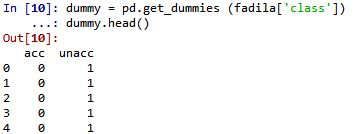
\includegraphics[scale=0.3]{figures/lanjutan1-1-fadila.jpg}
\caption{lanjutan1-1-fadila}
\label{lanjutan1-1-fadila}
\end{figure}
\par
\par
\begin{figure}[!hbtp]
\centering
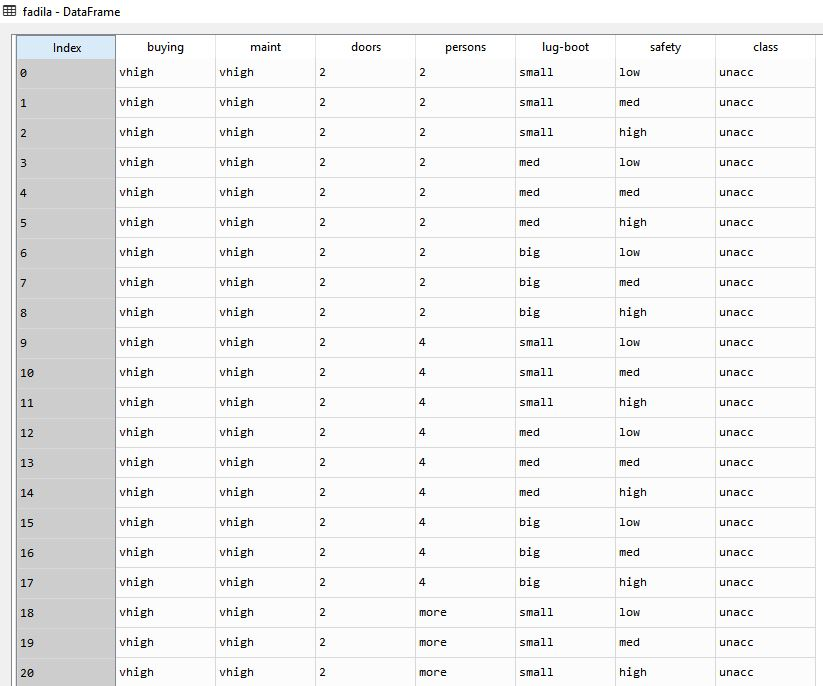
\includegraphics[scale=0.2]{figures/lanjutan1-2-fadila.jpg}
\caption{lanjutan1-2-fadila}
\label{lanjutan1-2-fadila}
\end{figure}
\end{itemize}
\par
\par
\item Pemecahan dataframe menjadi dua dataframe yaitu 450 row pertama dan 50 data sisa.
\begin{itemize}
\item Dataframe 1 : 450 row data pertama
\item Dataframe 2 : 50 row data sisanya.
\item Codingan Dan Penjelasannya :
\begin{lstlisting}
fadila_car_train = fadila_car[:450]
fadila_car_test = fadila_car[451:]
\end{lstlisting}
\begin{enumerate}
\item Baris 1 : Membuat variabel fadila\_car\_train dari variabel fadila\_car dengan 450 data awal untuk dijadikan data training
\item Baris 2 : Membuat variabel fadila\_car\_test dari variabel fadila\_car dengan 50 data sisanya untuk data testing ( dimulai dari data ke 451 sampai akhir data )
\end{enumerate}
\item Hasil Dari Pemecahan Dataframe
\par Penjelasan : Hasilnya dapat diliat pada gambar berikut \ref{2-fadila} dan \ref{lanjutan2-fadila}.
\begin{figure}[!hbtp]
\centering
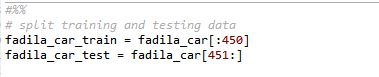
\includegraphics[scale=0.3]{figures/2-fadila.jpg}
\caption{2-fadila}
\label{2-fadila}
\end{figure}
\par
\par
\begin{figure}[!hbtp]
\centering
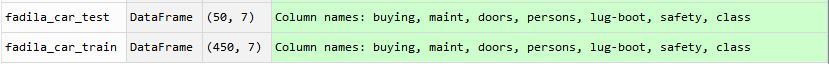
\includegraphics[scale=0.3]{figures/lanjutan2-fadila.jpg}
\caption{lanjutan2-fadila}
\label{lanjutan2-fadila}
\end{figure}
\par 
\par 
\end{itemize}
\par
\par
\item Vektorisasi Klasifikasi Data NPM mod 4 ( Katy Perry) Dengan Decision Tree
\par
\begin{lstlisting}
from sklearn import tree
clf = tree.DecisionTreeClassifier(criterion="entropy", max_depth=5)
clf = clf.fit(d_train_att, d_train_label)
\end{lstlisting}
\par Penjelasan : Sesuai Hasil.
\begin{enumerate}
\item Dalam [ in 21 ] merupakan hasil dari impor tree dari sklearn. Dan mendefinisikan variabel clf untuk memanggil Decission Tree Classifier dan melakukan fit atau pengujian.
\item Dalam [ in 22 ] menjelaskan bahwa digunakan prediksi untk clf dengan function predict untuk memprediksi test. Dan hasilnya muncul dalam bentuk array.
\item Kemudian Dalam [ in 23 ] clf score memunculkan akurasi prediksi yang dilakukan terhadap clf
\end{enumerate}
\par
\begin{itemize}
\item Hasil Program Menggunakan Decision Tree
\par Hasilnya dapat diliat pada gambar berikut \ref{3-fadila}.
\begin{figure}[!hbtp]
\centering
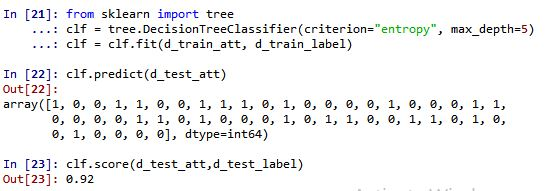
\includegraphics[scale=0.3]{figures/3-fadila.jpg}
\caption{3-fadila}
\label{3-fadila}
\end{figure}
\par
\par
\par
\end{itemize}
\par
\par
\item Vektorisasi Dengan Klasifikasi SVM
\par
\begin{lstlisting}
from sklearn import svm
clfsvm = svm.SVC()
clfsvm.fit(d_train_att, d_train_label)

clfsvm.score(d_test_att, d_test_label)
\end{lstlisting}
\par Penjelasan :
\begin{enumerate}
\item Dilakukan pengimportan module SVM dari sklearn
\item Selanjutnya melakukan fit dari d train att dan d train label atau disebut denga pengujian
\item Mendefinisikan variabel df untuk melakukan prediksi dataset Youtube Katy Perry dengan SVM. Dan akan muncul hasil prediksinya seperti pada contoh gambarnya
\end{enumerate}
\par
\begin{itemize}
\item Hasil Klasifikasi SVM
\par Hasilnya dapat diliat pada gambar berikut \ref{4-fadila}.
\begin{figure}[!hbtp]
\centering
\includegraphics[scale=0.3]{figures/4-fadila.jpg}
\caption{4-fadila}
\label{4-fadila}
\end{figure}
\par
\par
\par
\end{itemize}
\par
\par
\par
\item Vektorisasi Menggunakan Klasifikasi Decision Tree
\par
\begin{lstlisting}
from sklearn import tree
clf = tree.DecisionTreeClassifier()
clf = clf.fit(d_train_att, d_train_label)
clf.predict(d_test_att)
clf.score(d_test_att,d_test_label)
\end{lstlisting}
\par Penjelasan :
\begin{enumerate}
\item Dalam [ in 31 ] merupakan hasil dari impor tree dari sklearn. Dan mendefinisikan variabel clf untuk memanggil Decission Tree Classifier dan melakukan fit atau pengujian.
\item Di dalamnya juga menjelaskan bahwa digunakan prediksi untk clf dengan function predict untuk memprediksi test. Dan hasilnya muncul dalam bentuk array.
\item clf score memunculkan akurasi prediksi yang dilakukan terhadap clf
\item Lalu muncul lah hasilnya pada [ out 31 ] seperti pada gambar
\end{enumerate}
\begin{itemize}
\item Hasil Program Cross Validation
\par  Hasilnya dapat diliat pada gambar berikut \ref{5-fadila}.
\begin{figure}[!hbtp]
\centering
\includegraphics[scale=0.3]{figures/5-fadila.jpg}
\caption{5-fadila}
\label{5-fadila}
\end{figure}
\par
\par
\par
\end{itemize}
\par
\par
\item Plot Confusion Matrix
\begin{itemize}
\item Code Plot Confusion Matrix
\begin{figure}[!hbtp]
\centering
\includegraphics[scale=0.2]{figures/cod6-fadila.jpg}
\caption{cod6-fadila}
\label{cod6-fadila}
\end{figure}
\par Penjelasan : Untuk gambar \ref{cod6-fadila} yang ditampilkan / diperlihatkan telah dieksekusi dimana fungsi code tersebut yaitu untuk mencetak dan memplot Confussion Matrix. Normalisasi dapat diterapkan dengan mengatur `normalize = True`. Ada Confussion Matrik menggunakan normalisasi dan ada confussion matrik tidak menggunakan normalisasi.
\item Hasil Plot Confusion Matrix
\par Hasilnya dapat diliat pada gambar berikut \ref{6-fadila} dan \ref{lanjutan6-fadila} .
\begin{figure}[!hbtp]
\centering
\includegraphics[scale=0.2]{figures/6-fadila.jpg}
\caption{6-fadila}
\label{6-fadila}
\end{figure}
\par
\par
\begin{figure}[!hbtp]
\centering
\includegraphics[scale=0.25]{figures/lanjutan6-fadila.jpg}
\caption{lanjutan6-fadila}
\label{lanjutan6-fadila}
\end{figure}
\par
\end{itemize}
\par
\par
\item Program Cross Validation
\begin{lstlisting}
from sklearn.model_selection import cross_val_score
scores = cross_val_score(clf,d_train_att,d_train_label,cv=5)

skorrata2=scores.mean()
skoresd=scores.std()
\end{lstlisting}
\par Penjelasan :  Pada codingan maupun hasil dari cross validation berikut, menjelaskan dimana variabel score akan melakukan cross validation pada variabel clf, d train att, dan train label. Variabel skorrata2 akan menghitung nilai rata-rata dari variabel scores tadi menggunakan function mean. Dan scoresd menghitung standar deviasi dari data yang diberikan.
\begin{itemize}
\item Hasil Program Cross Validation
\par Hasilnya dapat diliat pada gambar berikut \ref{7-fadila} dan \ref{lanjutan7-fadila} .
\begin{figure}[!hbtp]
\centering
\includegraphics[scale=0.3]{figures/7-fadila.jpg}
\caption{7-fadila}
\label{7-fadila}
\end{figure}
\par
\begin{figure}[!hbtp]
\centering
\includegraphics[scale=0.3]{figures/lanjutan7-fadila.jpg}
\caption{lanjutan7-fadila}
\label{lanjutan7-fadila}
\end{figure}
\par
\end{itemize}
\par
\par
\par
\item Program Pengamatan Komponen Informasi
\begin{itemize}
\item Hasil Dan Code Pengamatan Komponen Informasi :
\par Hasilnya dapat diliat pada gambar berikut \ref{8-fadila} dan \ref{lanjutan8-fadila}.
\begin{figure}[!hbtp]
\centering
\includegraphics[scale=0.3]{figures/8-fadila.jpg}
\caption{8-fadila}
\label{8-fadila}
\end{figure}
\par
\par
\begin{figure}[!hbtp]
\centering
\includegraphics[scale=0.3]{figures/lanjutan8-fadila.jpg}
\caption{lanjutan8-fadila}
\label{lanjutan8-fadila}
\end{figure}
\par
\end{itemize}
\par Penjelasan :
\begin{enumerate}
\item Max featuresnya dari range 1 sampai 10
\item Untuk n estimators dengan range 2 sampai 40
\item Kemudian pada variabel rf params berisikan function np empty dimana akan membuat array baru berisikan tipe yang didefinisikan dengan random value
\item Mendefinisikan nilai i dimulai dari angka 0 dimana max features dan n estimators menggunakan klasifikasi randomforestclassifier menggunakan data prediksi.
\item Mendefinisikan rfparams untuk max features , n estimators, nilai rata dan std
\item Hasil (komponen informasi) juga ditampilkan dalam bentuk/module/ matplotlib
\item Secara keseluruhan untuk variabel x, y dan z dilakukan penyettingan dengan parameternya masing-masing
\item Label pun di definisikan untuk setiap variabelnya
\item Dan hasil keseluruhan akan nampak seperti pada gambar yang mengambarkan komponen informasi secara lengkap
\end{enumerate}
\par
\par
\par
\end{enumerate}


\par
\par
\par
\subsection{Penanganan Error Fadila}
Menangani dan Mengatasi Error Pada Praktek
\begin{enumerate}
\item Error 1 :
\begin{itemize} 
\item Code Yang Error :
\begin{lstlisting}
import pandas as pd
d = pd.read_csv("dataset/Youtube02-KatyPerry.csv")
\end{lstlisting}
\item Peringatan Error :
\begin{lstlisting}
FileNotFoundError: File b'dataset/Youtube02-KatyPerry.csv' does not exist
\end{lstlisting}
\item Gambar Error 1 : ( Lebih jelas )
\begin{figure}[!hbtp]
\centering
\includegraphics[scale=0.3]{figures/e1-fadila.jpg}
\caption{error1-fadila}
\label{error1-fadila}
\end{figure}
\begin{itemize}
\item Cara Penanganan :
\begin{enumerate}
\item Pada Codingan yang dieksekusi sebenarnya untuk membaca dataset dari Youtube02-KatyPerry.csv
\item Namun, terdapat error dan hal tersebut disebabkan karena file codingan yang dieksekusi tidak berada pada folder yang sama dengan dataset Katy Perry.
\item Silahkan tuliskan codingan berikut untuk mengganti codingan yang bermasalah
\begin{lstlisting}
import pandas as pd
d = pd.read_csv("Youtube02-KatyPerry.csv")
\end{lstlisting}
\item Dengan menganti codingan tersebut, maka tidak akan terjadi error lagi.
\par
\par
\end{enumerate}
\end{itemize}
\end{itemize}
\end{enumerate}


\subsection{Praktek}